\documentclass[acmlarge, screen, nonacm]{acmart}
\usepackage[utf8]{inputenc}
\usepackage{float}
\usepackage{setspace}
\usepackage{pgfplots}
\usepackage{graphicx}
\usepackage{fancyvrb}
\usepackage{listings}
\usepackage{xcolor}
\usepackage{ragged2e}
\usepackage{tikz}
  \usetikzlibrary{shapes}
  \usetikzlibrary{arrows.meta}
  \usetikzlibrary{arrows}
  \usetikzlibrary{shadows}
  \usetikzlibrary{trees}
  \usetikzlibrary{fit}
  \usetikzlibrary{calc}
  \usetikzlibrary{positioning}
  \usetikzlibrary{decorations.pathmorphing}
\definecolor{tikz-block}{HTML}{232527}
\tikzset{node distance=0.6cm, auto, every text node part/.style={align=center, font={\sffamily\small}}}
\tikzstyle{block} = [draw=tikz-block, fill=white, inner sep=0.3cm, outer sep=0.1cm, thick]
\tikzstyle{ln} = [draw, ->, very thick, arrows={-triangle 90}, every text node part/.append style={font={\sffamily\scriptsize}}]
\tikzstyle{O} = [circle, draw, every text node part/.style={align=center, font={\sffamily\small}}]
\usepackage{hyperref}
  \hypersetup{colorlinks=true,allcolors=blue!40!black}
\setlength{\topskip}{6pt}
\setlength{\parindent}{0pt} % indent first line
\setlength{\parskip}{6pt} % before par
% custom commands

\newcommand{\code}[1]{\texttt{#1}}
\newcommand{\todo}[1]{\textcolor{red}{TODO: #1}}

\title{GitLab commit protocol implementation}

\author{Ivan Bukhtiyarov}
\email{van4elotti@gmail.com}

\author{Kirill Chernyavskiy}
\email{g4s8.public@gmail.com}

\acmBooktitle{none}
\acmConference{none}
\editor{none}

\begin{document}

\begin{abstract}
  \emph{\href{https://gitlab.com/gitlab-org/gitaly}{Gitaly}}
  provides high-level RPC access to Git repositories. It is used by GitLab to read and write Git data.
  
  Current Gitaly Cluster architecture requires preventing unexpected data loss and organizing strong consistency (
  \emph{\href{https://gitlab.com/groups/gitlab-org/-/epics/1189}{Gitaly Cluster: strong consistency}}).
  Due to experiments that are related to this problem
  \emph{\href{https://gitlab.com/gitlab-org/gitaly/-/issues/2466}{Implement 3PC for WriteRef RPC}},
  \emph{\href{https://gitlab.com/gitlab-org/gitaly/-/issues/2529}{3PC git-update-ref experiment}} and
  \emph{\href{https://gitlab.com/gitlab-org/gitaly/-/issues/2635}{2PC via pre-receive hook}}
  it was suggested that GitLab probably uses three-phase commit (3PC) protocol for managing atomic transactions. 
  But 3PC and any other commit protocols has many different implementations and
  additional extensions (such as recovery and termination protocols): it means that protocols could
  be implemented differently depends on business requirements. In this report we analyze what
  components of commit protocol is used by GitLab and how it achieves (or doesn't achieve) 
  strong consistency, by describing the whole workflow of each git push command from 
  client to replicas and investigating extension protocols for dealing with node and network failures.
\end{abstract}

\maketitle

\section{Introduction}

Gitlab team pays attention on fact that number of users, repositories, and activity grows, it is important to scale Gitaly appropriately by:

\begin{enumerate}
\item Increasing the available CPU and memory resources available to Git before resource
exhaustion degrades Git, Gitaly, and GitLab application performance.
\item Increase available storage before storage limits are reached causing write operations to fail.
\item Improve fault tolerance by removing single points of failure. Git should be considered
mission critical if a service degradation would prevent you from deploying changes to production.
\end{enumerate}

Current Degitx team's research goal is to find the most relevant protocol to achieve 
strong consistency in Degitx distributed git repository manager. The technical report is the part of this complex research, 
where we analyse the most successful open source solution of distributed repository manager project.
Despite the fact that the Gitaly team claims strong consistency, the commit protocol in current Gitaly 
implementation can have some disadvantages. The main goals of this technical report are : 
\begin{itemize}
\item to describe full Gitlab workflow of some mutator operation like ``git push'' 
\item to figure out the distribute fetch process 
\item to find possible cases when inconsistency can be hit 
\item to describe Gitaly protocol's advantages and disavanges to production usage. 
\end{itemize}
 
\section{Gitlab consistency}
  Achieving strong consistency in gitaly is dedicated to an
  \emph{\href{https://gitlab.com/groups/gitlab-org/-/epics/1189}{epic}}. 
  that includes a set of issues. Some of tickets were successfully implemented and integrated,
  some of them remained on POC stage or simply closed.
  
  Curent Gitaly Cluster allows Git repositories to be replicated on multiple Gitaly nodes. 
  This improves fault tolerance by removing single points of failure. 
  Reference transactions causes changes to be broadcast to all the Gitaly nodes in the cluster, 
  but only the Gitaly nodes that vote in agreement with the primary node persist the changes to disk. 
  If all the replica nodes dissented, only one copy of the change would be persisted to disk, 
  creating a single point of failure until asynchronous replication completed.

  Quorum-based voting improves fault tolerance by requiring a majority of nodes 
  to agree before persisting changes to disk. Dissenting nodes are automatically brought in sync by
   asynchronous replication from the nodes that formed the quorum.

  As for \emph{\href{https://gitlab.com/groups/gitlab-org/-/epics/1189}{praefect}}, it can configured 
  with one of two types of consistency:
  \begin{description}
    \item[Eventual concistency]
    Praefect guarantees eventual consistency by replicating all writes 
    to secondary nodes after the write to the primary Gitaly node has happened.
    \item[Strong concistency]
    Praefect can instead provide strong consistency by creating a transaction and writing
     changes to all Gitaly nodes at once. If enabled, transactions are only available for a subset of RPCs. 
  \end{description}
  
\section{Accessor and mutator RPCs}
Gitaly provides RPC access to Git repositories. It is used by GitLab to read and write Git data from repositories.
Gitaly clients (Gitlab Rails, shell or Workhorse) make requests of the Gitaly server.  Praefect \textbf{ensures} 
that all gRPC calls from clients, that were mentioned before, are forwarded to the correct shard by consulting the
\emph{\href{https://gitlab.com/gitlab-org/gitaly/-/blob/master/internal/praefect/coordinator.go}{coordinator}}.

Gitaly RPCs are divided on groups:
\begin{itemize}
\item Accessor - read-only RPC, that does not modify the git repository.
\item Mutator - an RPC that modifies the data in the git repository.
\end{itemize}

Mutator operation workflow described at the Fig.\ref{fig:push-workflow}

Moreover some acessor RPCs like \textit{GetObjectDirectorySize} or \textit{RepositorySize} have \textbf{\textit{forcePrimary}} flag. 
Coordinator server router handle accessor RPCs with  
\emph{\href{https://gitlab.com/gitlab-org/gitaly/-/blob/master/internal/praefect/coordinator.go\#L356}{ RouteRepositoryAccessor}}. 
It returns the node that should serve the repository accessor request. If \textbf{\textit{forcePrimary }} is set to `true`, it returns the primary node. 
If it set to `false`: 
\begin{enumerate}
\item Finds all UpToDate storages (according the generation number that is written in the database).
\item Choose only healthy ones.
\item Return some random node from this set.
\end{enumerate}

\section{Gitlab mutator operation Workflow}
There are multiple components involved into git replication protocol workflow:
\begin{enumerate}
    \item Client --- git client who performce push and fetch operations
    \item Workhorse --- component exposes HTTP endpoint to accept
      git client requests and translate to internal RPC protocol
    \item Shell --- component exposes SSH port and accept client
      SSH git commands, then translate to internal RPC protocol
    \item Rails --- main GitLab application, it provides web user-interface
      and exposes internal API. Workhorse and Shell uses Rails
      for discovery: when git client performs some operation,
      they uses Rails to find proper RPC node to talk.
    \item Gitaly --- git repository resource manager (RM): it provides RPC
      for all git operations and calls git or libgit to manage
      the repository. There are many Gitaly nodes in GitLab cluster,
      each repository is replicated to multiple nodes for availability
      and fault-tolerance.
    \item Praefect --- A proxy and transaction manager (TM) for Gitaly. It handles
      incoming RPC requests to Gitaly and redirect it to correct one.
      Also, it works as a TM in two phase commit transaction by exposing
      \code{vote} methods for RMs.
    \item Git --- a git process performing repository updates, it's started by
      Gitaly on RPC calls and trigger some hooks which helps with transaction
      management. It's located on same node as Gitaly process.
    \item Hook --- git reference transaction hook, it's triggers by Git,
      notify transaction status to Gitaly, and blocking wait to signal from
      Gitaly to exit and unlock the Git process on transaction.
\end{enumerate}

\begin{figure}
  \begin{center}
    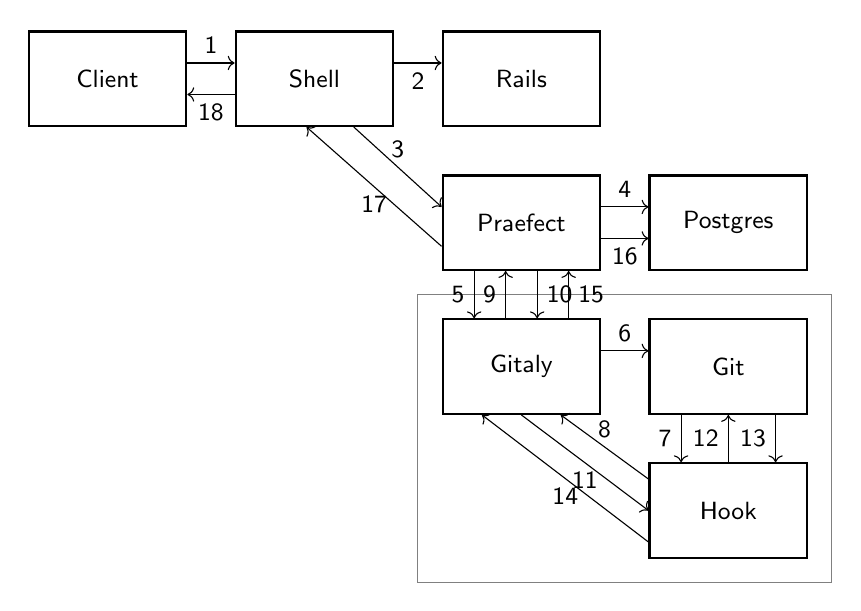
\begin{tikzpicture}[
        wide-block/.style={rectangle, draw=black, fill=white, thick, minimum width=2cm, minimum height=1.2cm},
        half-wide-block/.style={rectangle, draw=black, fill=white, thick, minimum width=2cm, minimum height=1.2cm},
        group-node/.style={rectangle, draw=gray, inner sep=0.3cm}
      ]
      \node[wide-block]        (cli)                           {Client};
      \node[wide-block]        (shell)[right=of cli]           {Shell};
      \node[wide-block]        (rails)[right=of shell]         {Rails};
      \node[wide-block]        (pkt)[below=of rails]           {Praefect};
      \node[wide-block]        (pg)[right=of pkt]              {Postgres};
      \node[wide-block]        (gly)[below=of pkt]             {Gitaly};
      \node[wide-block]        (git)[right=of gly]             {Git};
      \node[wide-block]        (hook)[below=of git]            {Hook};
      \node[group-node]        (rm)    [fit=(gly)(git)(hook), label={}] {};
      \draw[->]                ($(cli.east)+(0,0.2)$)            -- node[above] {1}     ($(shell.west)+(0,0.2)$);
      \draw[->]                ($(shell.east)+(0,0.2)$)            -- node[below] {2}     ($(rails.west)+(0,0.2)$);
      \draw[->]                ($(shell.south)+(0.5,0)$)            -- node[above] {3}     ($(pkt.west)+(0,0.2)$);
      \draw[->]                ($(pkt.east)+(0,0.2)$)            -- node[above] {4}     ($(pg.west)+(0,0.2)$);
      \draw[->]                ($(pkt.south)+(-0.6,0)$)            -- node[left] {5}     ($(gly.north)+(-0.6,0)$);
      \draw[->]                ($(gly.east)+(0,0.2)$)            -- node[above] {6}     ($(git.west)+(0,0.2)$);
      \draw[->]                ($(git.south)+(-0.6,0)$)            -- node[left] {7}     ($(hook.north)+(-0.6,0)$);
      \draw[->]                ($(hook.west)+(0,0.4)$)            -- node[above] {8}     ($(gly.south)+(0.5,0)$);
      \draw[->]                ($(gly.north)+(-0.2,0)$)            -- node[left] {9}     ($(pkt.south)+(-0.2,0)$);
      \draw[->]                ($(pkt.south)+(0.2,0)$)            -- node[right] {10}     ($(gly.north)+(0.2,0)$);
      \draw[->]                ($(gly.south)+(0,0)$)            -- node[below] {11}     ($(hook.west)+(0,0)$);
      \draw[->]                ($(hook.north)+(0,0)$)            -- node[left] {12}     ($(git.south)+(0,0)$);
      \draw[->]                ($(git.south)+(0.6,0)$)            -- node[left] {13}     ($(hook.north)+(0.6,0)$);
      \draw[->]                ($(hook.west)+(0,-0.4)$)            -- node[below] {14}     ($(gly.south)+(-0.5,0)$);
      \draw[->]                ($(gly.north)+(0.6,0)$)            -- node[right] {15}     ($(pkt.south)+(0.6,0)$);
      \draw[->]                ($(pkt.east)+(0,-0.2)$)            -- node[below] {16}     ($(pg.west)+(0,-0.2)$);
      \draw[->]                ($(pkt.west)+(0,-0.3)$)            -- node[below] {17}     ($(shell.south)+(-0.1,0)$);
      \draw[->]                ($(shell.west)+(0,-0.2)$)            -- node[below] {18}     ($(cli.east)+(0,-0.2)$);
    \end{tikzpicture}
  \end{center}
  \caption[GitLab repository push workflow]{
    GitLab repository push workflow} {
    \begin{flushleft}
    1. Git client calls shell (or workhorse);
    2. Shell find Gitaly shard in Rails;
    3. Shell calls Praefect to accept git pack; 
    4. Praefect search database for valid Gitaly nodes for repository;
    5. Praefect calls all Gitaly RPC to accept git pack;
    6. Each Gitaly node starts git process to apply pack; 
    7. Git apply pack and exec reference transaction hook with metadata;
    8. Hook notify Gitaly that pack could be applied with ``prepared'' message,
    and start waiting for the response;
    9. Each Gitaly notify Praefect by voting on transaction;
    10. Praefect waits for quorum of Gitaly nodes with prepared vote and
    send ``commit'' command to each of them;
    11. Gitaly respond to Hook with commit response;
    12. Hook exits with zero status and unlock Git, which can apply the transaction;
    13. Git apply transaction and unlock references, notify Hook with ``commited'' message,
    and finish the process (exit);
    14. Hook notyfy Gitaly that transaction was commited.
    15. Gitaly notify Praefect that transaction was commited;
    16. Praefect increment Gitaly version in database on commit finished;
    17. When all Gitaly nodes send ``commited'', Praefect respond to Shell with success status;
    18. Shell respond to Git client that push was successful;
    \end{flushleft}
  }\label{fig:push-workflow}
\end{figure}
\section{3PC}


Due to current status of code research and the facts from these 
(\emph{\href{https://gitlab.com/gitlab-org/gitaly/-/issues/2466}{Implementation 3PC for WriteRef RPC}},
\emph{\href{https://gitlab.com/gitlab-org/gitaly/-/issues/2529}{3PC git-update-ref experiment}})
POCs we can assume that the three-phase commit is not implemented in gitlab at all.

3PC for WriteRef was suggested in this
\emph{\href{https://gitlab.com/gitlab-org/gitaly/-/issues/2466}{MR}},
but it was not merged to actual branches. (All the reasons are in the process of clarification)

\section{Recovery protocol}

\subsection{SQL primary election strategy}
\emph{\href{https://gitlab.com/gitlab-org/gitaly/-/blob/master/internal/praefect/nodes/sql_elector.go}{sqlElector }}manages the primary election for one virtual storage (aka
shard). It enables multiple, redundant Praefect processes to run,
which is needed to eliminate a single point of failure in Gitaly High
Avaiability.

The sqlElector is responsible for:
\begin{itemize}
\item Monitoring and updating the status of all nodes within the shard.
\item Electing a new primary of the shard based on the health.
\end{itemize}
Also every Praefect node periodically performs a health check RPC with a Gitaly node.  Once the health checks are complete, 
Praefect node does a \textit{SELECT} from \textit{node\_status} table to determine healthy nodes.
The primary of each shard is listed in the
\textit{shard\_primaries}. If the current primary is in the healthy
node list, then \textit{sqlElector} updates its internal state to match.

Otherwise, if there is no primary or it is unhealthy, any Praefect node
can elect a new primary by choosing candidate from the healthy node
list. Gitaly uses repository generations to determine the best leader to elect.  

\subsection{Repository generations }

Praefect records the expected latest generation of each repository  in \textit{repositories } table.

We have generations for each repository we could use this info to determine a new primary node more efficiently and correctly. 
The new primary is the one that has less generation delay in total for all repositories. If there is no data to determine the 
primary in the database the \textbf{first} candidate in candidate list (healthy nodes) will be the new primary.

Generation increment algo (\emph{\href{https://gitlab.com/gitlab-org/gitaly/-/blob/master/internal/praefect/datastore/repository_store.go}{Gitaly code}}) :
\begin{enumerate}
\item Increment the latest generation. If no previous records exists, the generation starts from 0.
\item Get the primary's current generation. Secondaries have to be on the primary's generation at the moment of increment. 
This avoids any issues where a concurrent reference transaction has failed and the secondary is no longer up to date when 
we are incrementing the generations.
\item Filter out secondaries which participated in a transaction but failed a concurrent transaction.
\item Combine the primary and the up to date secondaries in a list of storages to increment the generation for.
\item Update table with new generations for this pimary and up to date secondaries.
 \end{enumerate}
If there are no candidate nodes, the primary is demoted by setting the \textit{demoted} flag in \textit{shard\_primaries}.

In case of a failover, the virtual storage is marked as read-only until writes are manually enabled
again. This status is stored in the \textit{shard\_primaries} table's \textit{read\_only }column. 
If \textit{read\_only } is set, mutator RPCs against the storage shard should be blocked. This procedure is made 
to prevent creating new primary node before data recovery attempts have been made.

The different scenarios of node failures described \emph{\href{https://gitlab.com/gitlab-org/gitaly/-/blob/master/internal/praefect/nodes/sql_elector.go\#L401}{in the code comments}}.

Currently Praefect (TM) don't support the failover on other Praefect node in case of its failure during the transaction.

\subsection{Virtual storages}

Distributed nature of the storage cluster is hidden from the client by exposing an interface that looks like a single storage.
In Praefect, this abstraction is called \emph{\href{https://gitlab.com/gitlab-org/gitaly/-/blob/master/doc/virtual_storage.md}{ virtual storage}}. 
Each virtual storage has one or more physical storages, the Gitaly nodes. 

Praefect records the expected state of each repository within a virtual storage in the \textbf{repositories} table

\textbf{repositories} table

 \begin{tabular}{||c c c ||} 
 \hline
 virtual\_storage &relative\_path & generation  \\ [0.5ex] 
 \hline\hline
 default & @hashed/5f/9c/5f9c4a...b08ca.git & 5\\  
 \hline
\end{tabular}

Praefect tracks the current state of a repository on each physical storage in the storage\_repositories table:

\textbf{storage\_repositories} table

 \begin{tabular}{||c c c c||} 
 \hline
 virtual\_storage &relative\_path & storage & generation  \\ [0.5ex] 
 \hline\hline
 default & @hashed/5f/9c/5f9c4a...b08ca.git& gitaly-1 & 5\\  
 \hline
 default & @hashed/5f/9c/5f9c4a...b08ca.git & gitaly-2 & 5\\  
 \hline
\end{tabular}


With reference transactions, healthy secondaries on the same generation as the primary participate in the transaction 
together with the primary. On transaction completion, Praefect atomically increments the generation counter in
\textbf{repositories} and sets the primary's generation to match it in \textbf{storage\_repositories}. 
Secondaries' generations are only incremented if they were on the same generation as the primary at the 
time of the increment. This is to avoid incrementing the generation number for secondaries that 
failed a concurrent transaction.


\section{Termination protocol}

In \emph{\href{https://gitlab.com/gitlab-org/gitaly/-/tags/v14.0.0-rc1}{ current}} 
Gitaly version there is 5 minutes transaction timeout that is set on transaction 
context when voting client on gitaly node votes on transaction (the voting client 
communicates with Praefect node).
The timeout used for all transactional actions like voting and stopping of transactions.
 The reasons of setting of this long timeout you can find 
In \emph{\href{https://gitlab.com/gitlab-org/gitaly/-/blob/master/internal/gitaly/transaction/manager.go\#L21}{ source code comments}}. 
In other words It shouldn't normally be hit, but if it is hit then it indicates that Praefect still waiting to the quorum reaching. 

For gitaly clients it means that it can be waiting around for up to 5 minutes while the transaction 
is completing if in case votes are missing to reach the quorum.

There no any other timeouts on Praefect node or reference transaction hook side. 
Hook will be waiting the any end scenario of transaction. They are :

\begin{itemize}
\item Transaction commited.
\item Transaction stopped indicates a transaction was gracefully stopped. 
This only happens in case the transaction was terminated because of an external condition, e.g. access 
checks or hooks rejected a change.
\item Transaction aborted indicates a transaction was aborted, either because it timed out or because 
the vote failed to reach quorum.
\item Invalid transaction state.
\end{itemize}

\section{Gitaly problems}
This section introduces some Gitaly issues that realated to our research topics. Some 
of this scenarios can be useful for future protocol testing different scenarios. 
\begin{itemize}
\item  \emph{\href{https://gitlab.com/gitlab-org/gitaly/-/issues/3605}{ Failed changes when primary is down still increment 
generation and cause repo to become read-only}}. It describes the scenario when Gitaly node has gone down but is still 
considered primary by Praefect, mutator requests received during this period will increment the generation column 
in \textit{storage repositories} table.
\item  \emph{\href{https://gitlab.com/gitlab-org/gitaly/-/merge_requests/3494}{ MR about considering the primary node modified}}. 
The ideas in this MR can be studied to find inconsistency scenarios that changes cannot solve.
\item  \emph{\href{https://gitlab.com/gitlab-org/gitaly/-/blob/master/doc/virtual\_storage.md\#known-problems}{Gitaly team known problems}} 
that connected with sql primary election strategy. 
\end{itemize}

After Gitaly commit protocol analysis, was noticed that the incrementing of generation in \textit{repositories} 
and \textit{store\_repositories} tables happens after Praefect (TM) 
response to Gitaly (RM) on \textit{VoteTransactionRequest}. If the TM crashes 
after sending \textit{Commit} response to Gitaly nodes and before transaction 
finalizer that calls incrementing mentioned above we can hit the situation:
	
\begin{enumerate}
\item Transaction was successfully finished because of quorum was reached.
\item Some Gitaly nodes aborted transaction, and became outdated.
\item Generations of all Gitaly nodes that was participated in transaction remained the same, because of Praefect failure before its incrementing.
\item The result: Gitaly nodes that failed the transaction and successfully participate in it have the \textbf{same} an old generation number. In other words some Gitaly nodes have different data but the same generation.
\end{enumerate}


\section{Conclusion and future work}

Analysis of Gitlab commit protocol and Gitaly workflow shows that Gitlab commit protocol in most cases
copes with achieving strong consistency. Despite that 
fact, some disadvantages can be noticed in Gitaly approach:
\begin{itemize}
\item Possible deadlock while the transaction is completing in case votes are missing to reach the quorum.
\item High Gitaly project complexity (using sql election strategy, virtual storages).
\item To achieve Postgres high availability in this approach need to use additional resources PostgreSQL cluster and HAProxy. 
\end{itemize}
The future research will be aimed to possibility of replacing Giltaly commit protocol (modified 2pc) 
with the \emph{\href{https://en.wikipedia.org/wiki/Paxos_(computer_science)}{Paxos}}. This approach can help us to achieve 
a strong consistency in an easier way in distributed git repository manager Degitx.

\end{document}